    \documentclass[
%	msc, %% Para dissertações de mestrado, OU
	mscproposta, %% Para propostas de dissertação de mestrado, OU
%	phd, %% Para teses de doutorado, OU
%	phdproposta, %% Para propostas de tese de doutorado
%	portugues %% Para documentos em português, OU
	english %% Para documentos em inglês
]{../ppgccufmg}

%\usepackage[brazil]{babel} %% se o documento for em português, OU
\usepackage[english]{babel} %% se o documento for em inglês
%\usepackage[latin1]{inputenc}
\usepackage[numbers,sort&compress]{natbib}
\usepackage{xcolor}
\usepackage{lipsum}

%% A classe ppgccufmg já carrega o hyperref internamente (necessário para
%% gerar PDF/A). Não use \usepackage{hyperref} aqui -- configure as opções
%% do pacote com \hypersetup{} (veja o README para mais detalhes).
\hypersetup{
	colorlinks=true,
	linkcolor=blue, %% Cor dos links do sumário
	citecolor=red, %% Cor dos links das citações
	urlcolor=magenta, %% Cor das urls
}

%% Exemplo 1 de lista customizada: Glossário ==================

\newcommand{\glossario}{
	\chapter*{List of Abbreviations and Acronyms}
	
	\begin{tabular}{ll}
		BFS & \textit{Breadth-First Search}\\
		BOW & \textit{Bag of Words} \\
		TXT & \textit{Text File Format}\\
		UFMG & Universidade Federal de Minas Gerais
	\end{tabular}
}

%% **** Caso não haja nenhuma lista adicional, os comandos acima podem ser apagados. ****
%% ===============================================

%% Exemplo 2 de lista customizada: Lista de algoritmos ==================
%% Para criar uma lista customizada (como Lista de Algoritmos, Lista de Exemplos) que ficará juntamente com as Lista de Figuras e Lista de Tabelas, execute os 3 comandos abaixo substituindo "algoritmos" pelo tipo de lista que estará criando. Para adicionar a lista ao documento, deverá passar o seguinte parâmetro no comando \ppgccufmg:
%% \ppgccufmg{
%% 		...
%% 		listacustomizada={\listadealgoritmos}
%% }
%\newfloat[chapter]{algoritmo}{lol}{Algoritmo}
%\newcommand{\listaalgoritmosname}{Lista de Algoritmos} %% Título da lista
%\newlistof{listadealgoritmos}{lol}{\listaalgoritmosname} %% O primeiro parâmetro é o nome da lista, e este deverá ser passado no parâmetro listacustomizada={\nomedalista}
%\newlistentry{algoritmo}{lol}{0} %% Nome do ambiente de cada algoritmo, e.g., \begin{algoritmo} ... \end{algoritmo}

%% **** Caso não haja nenhuma lista adicional, os comandos acima podem ser apagados. ****
%% ===============================================


\begin{document}
	\ppgccufmg{
		autor={Guilherme Silva Toledo}, %% Autor(a)
		titulo={Semantics-Aware Gaussian Splatting for Egocentric Hyperlapse}, %% Título
		cidade={Belo Horizonte},
		ano={2026},
		versao={Draft}, %% Versão do documento
		orientador={Erickson Rangel do Nascimento}, %% Para masculino
		% orientadora={Fulana de Tal}, %% Para feminino
		% coorientador={Ciclano}, %% Para masculino
		% coorientadora={Ciclana}, %% Para feminino
		% fichacatalografica={fichacatalografica.pdf},
		% folhadeaprovacao={folhadeaprovacao.pdf},
		resumo={resumo.tex}, %% Resumo em português
		abstracten={abstract.tex}, %% Abstract em inglês
		palavraschave={Hyperlapse semântico. Gaussian splatting. Vídeo egocêntrico. Síntese de novas vistas.}, %% Palavras-chave do resumo
		keywords={Semantic hyperlapse. Gaussian splatting. Egocentric video. Novel view synthesis.}, %% Palavras-chave do abstract
		% dedicatoria={dedicatoria.tex}, %% Arquivo .tex contendo a dedicatória
		% agradecimentos={agradecimentos.tex},
		% epigrafe={Truth and lie are opposite things.},
		% epigrafeautor={Unkown},
		% listadefiguras={sim}, %% Remova (ou comente) este parâmetro para remover a lista de figuras
		% listadetabelas={sim}, %% Remova (ou comente) este parâmetro para remover a lista de tabelas
		% listascustomizadas={\glossario} %% Lista customizada (e.g., glossário, lista de algoritmos). 
	}
	
	% \chapter{Tema e Justificativa(Introdução)}
	% 	Exemplo de nota de rodapé \footnote{Aqui está uma nota de rodapé e uma url: \url{https://dcc.ufmg.br}}.
	% 	\lipsum[1-4]
		
	% 	\section{Motivação}
	% 		\lipsum[4-5]
			   
	% 		\subsection{Sub-motivação}
	% 			\lipsum[6-7]
	% 		\subsection{Mais uma sub-motivação}
	% 			\lipsum[8-9]
	% 			\subsubsection{Uma sub-sub-motivação}
	% 				\lipsum[10-11]
	
% 	\chapter{Objetivos(Desenvolvimento)}
% 		\lipsum[1-4]
		
% %		Exemplo de algoritmo ==============================
% %		\begin{algoritmo}
% %			\centering
% %			\framebox[.5\textwidth]{\texttt{Código, Código, Código}}
% %			\caption{Este é o meu Algoritmo 1.}
% %			\label{alg:algoritmo1}
% %		\end{algoritmo}
% %	
% %		\begin{algoritmo}
% %			\centering
% %			\framebox[.7\textwidth]{\texttt{Mais Código, Mais Código, Mais Código}}
% %			\caption{Este é o meu Algoritmo 2.}
% %			\label{alg:algoritmo2}
% %		\end{algoritmo}
% %		===============================================
		
% 		\begin{figure}[ht]
% 			\centering
% 			\caption{Prédio do DCC em 2016.}
% 			\label{fig:exemplo}
% 			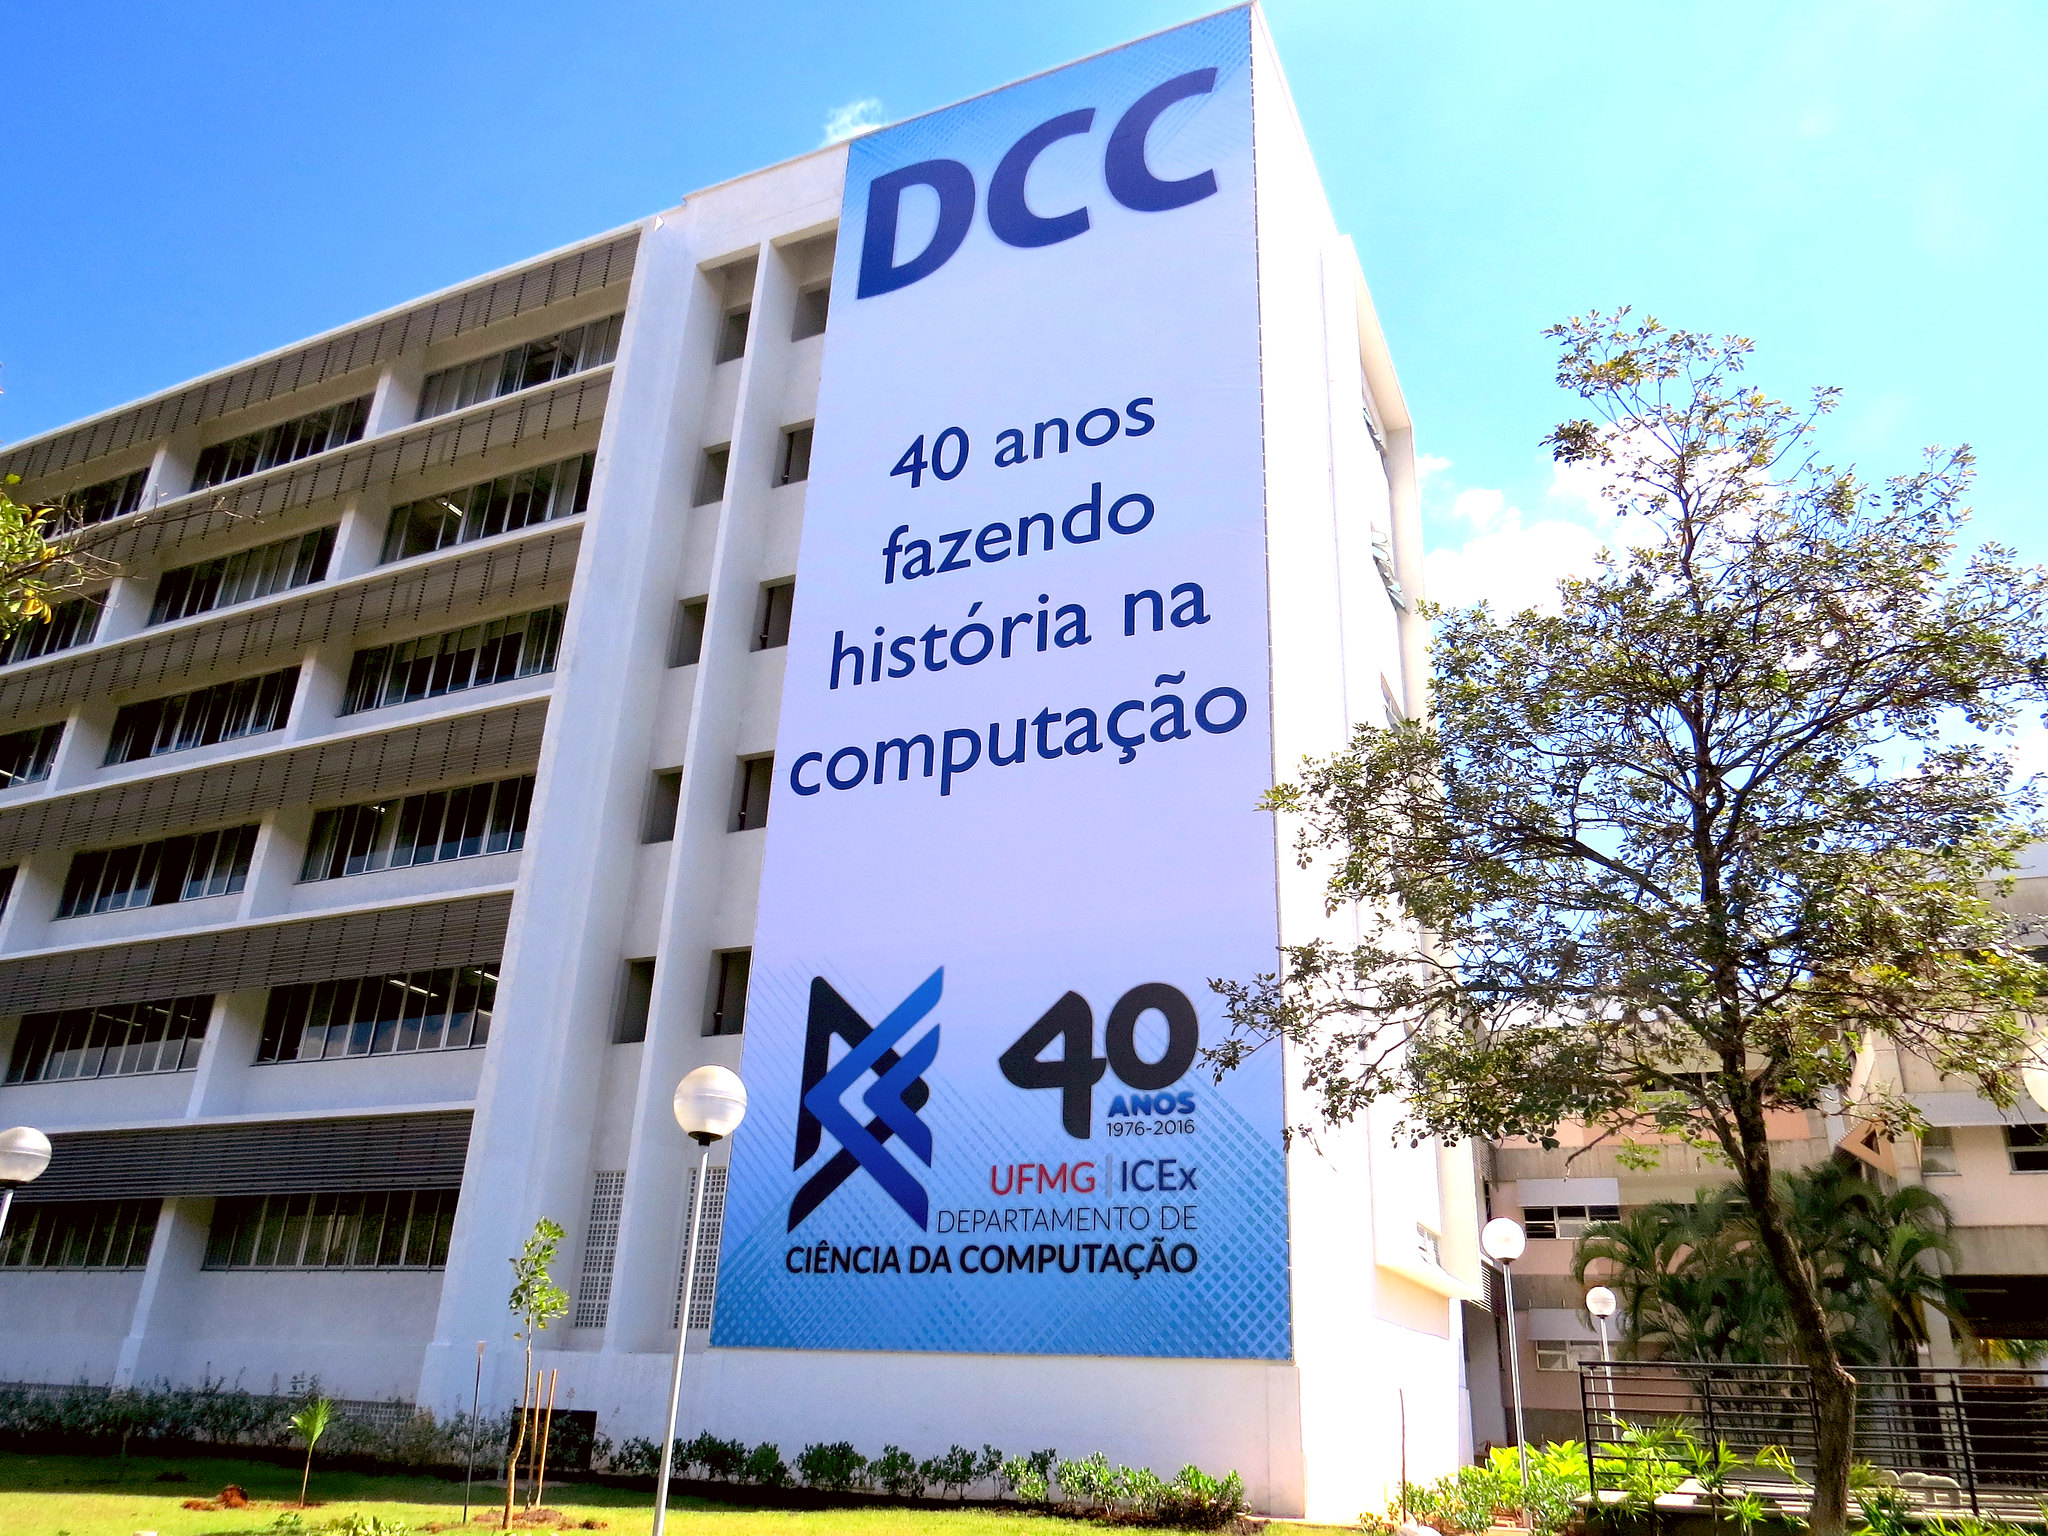
\includegraphics[width=\textwidth]{img/dcc.jpg}
% 			\small{Fonte:~\url{http://40anos.dcc.ufmg.br/galeria}}
% 		\end{figure}
	
% 		\lipsum[5]
		
% 		\begin{table}[ht]
% 			\centering
% 			\begin{tabular}{c|ccccccccl}
% 				Natural & \multicolumn{9}{c}{Real}   \\ \hline
% 				1 & 0.  & {\color{red} 2}  & 3   & 6   & 4   & 3   & 6   & 7   & $\ldots$ \\
% 				2  & 0.  & 0   & {\color{red} 9}  & 8   & 4   & 7   & 3   & 2   & $\ldots$ \\
% 				3  & 0.  & 1   & 9   & {\color{red} 3}  & 2   & 1   & 4   & 0   & $\ldots$ \\
% 				4  & 0.  & 8   & 4   & 3   & {\color{red} 2}  & 7   & 9   & 2   & $\ldots$ \\
% 				5  & 0.  & 0   & 1   & 2   & 9   & {\color{red} 3}  & 4   & 8   & $\ldots$ \\
% 				6  & 0.  & 2   & 8   & 2   & 6   & 5   & {\color{red} 8}  & 3   & $\ldots$ \\
% 				7  & 0.  & 0   & 2   & 1   & 5   & 3   & 7   & {\color{red} 4}  & $\ldots$ \\
% 				$\vdots$ & $\vdots$  & $\vdots$  & $\vdots$  & $\vdots$  & $\vdots$  & $\vdots$  & $\vdots$  & $\vdots$  & $\ddots$ \\ \hline
% 				\multicolumn{1}{l|}{} & \multicolumn{1}{l}{0.} & \multicolumn{1}{l}{{\color{red} 2}} & \multicolumn{1}{l}{{\color{red} 9}} & \multicolumn{1}{l}{{\color{red} 3}} & \multicolumn{1}{l}{{\color{red} 2}} & \multicolumn{1}{l}{{\color{red} 3}} & \multicolumn{1}{l}{{\color{red} 8}} & \multicolumn{1}{l}{{\color{red} 4}} & $\ldots$
% 			\end{tabular}
% 			\caption{Cantor: Existem infinitos diferentes!}
% 			\label{tab:exemplo}
% 		\end{table}

% 		\section{Usando referências}
% 			Segundo \cite{horn86robot}, todo triângulo equilátero tem os lados iguais. Já segundo \cite{shashua97photometric}, todo quadrado também tem.
			
% 			Veja que o pacote \verb|natbib| permite uma série de formas diferentes para fazer referências bibliográficas. O comando padrão, \verb|\cite|, realiza a citação comum vista no parágrafo anterior. Outros comandos permitem, por exemplo, colocar automaticamente a citação entre	parênteses \citep{hougen93estimation, sato99illumination2, sato99illumination1, sato01stability}.
			
% 			O comando usado foi \verb|\citep|. Veja a documentação do \verb|natbib| na Internet para conhecer	outros comandos e exemplos de uso.
			
% 			Citações aleatórias para fazer com que as referências bibliográficas ocupem	mais de uma página: \cite{bichsel92simple, dror01statistics, guisser92new, dwork2006calibrating, sweeney2002k}.
			

    \setlength{\afterchapskip}{0.6cm}
    \chapter{}
    \section{Theme and explanation}
        Wearable cameras such as the Project Aria glasses~\cite{engel2023aria} can record hours of useful activity, but direct temporal subsampling amplifies head motion and may remove the moments that explain an event. Semantic hyperlapse addresses the second problem by assigning relevance to frames and varying the speed-up along the video~\cite{ramos2016fastforward}. Sparse semantic sampling preserves relevant content while controlling instability and output duration~\cite{silva2018weighted,silva2021sparse}. Text-driven methods further show that relevance can be learned from language and optimized through sequential decisions~\cite{ramos2020straight,ramos2022text}. Emitting only recorded frames, these methods repair smoothness afterwards with stabilization and transition smoothing~\cite{silva2016towards,silva2018weighted}. They mainly choose among captured frames and reason mostly in image space, so they cannot place the output camera at a viewpoint that was not recorded, and semantic retention and visual smoothness remain coupled to the original shaky path.

        Geometric hyperlapse follows a complementary direction. First-person Hyperlapse reconstructs the input trajectory, optimizes a smoother virtual camera path, and synthesizes its views from nearby frames~\cite{kopf2014hyperlapse}. Recent 3D Gaussian Splatting (3DGS) represents a scene with explicit anisotropic primitives and renders high-quality novel views in real time~\cite{kerbl2023gaussian}. Lv et al.~\cite{lv2025photoreal} adapted it to egocentric devices, modelling rolling shutter and high dynamic range on Aria recordings; its code has already been run on the entire Aria dataset for this project.

        Language-embedded variants attach open-vocabulary features to this representation. LangSplat compresses CLIP features and learns object boundaries from SAM masks~\cite{qin2024langsplat}; Semantic Gaussians projects features from several image encoders into an existing splat~\cite{guo2024semantic}; and EgoSplat adds multi-view instance aggregation and transient filtering for egocentric video~\cite{li2025egosplat}. EgoLifter similarly shows that object instances can be lifted from egocentric images into 3D~\cite{gu2024egolifter}.

        Relevance can therefore be defined in 3D, on the representation that is rendered, although egocentric splats remain worse than exocentric ones~\cite{warchocki2026personal}. No prior work plans a hyperlapse camera path over a semantic Gaussian scene; this proposal fills that gap: a semantic hyperlapse in which Gaussian-splat reconstruction provides the geometry and open-vocabulary semantics, and a path-planning stage uses that spatial-semantic model to render a smooth, fast, semantically faithful first-person video.
    \section{Goals}
        The main objective is to integrate Gaussian splatting into the semantic hyperlapse pipeline, making novel view synthesis available as in Kopf et al.~\cite{kopf2014hyperlapse} and decisions spatial-semantic rather than frame-wise. The specific objectives are: (i) lift open-vocabulary semantics onto the completed egocentric reconstructions, following EgoSplat~\cite{li2025egosplat}, so that per-Gaussian relevance is queried in 3D; (ii) formulate semantic virtual camera path planning as a smooth trajectory maximizing accumulated relevance at a target speed-up, trading off proximity to the original trajectory and rendering quality; (iii) render that trajectory from the Gaussians, lifting the recorded-frame constraint that forces 2D methods to repair smoothness; and (iv) compare against both families on smoothness, semantics and motion fluidity.
    \section{Methodology}
        \textbf{Reconstruction and replication.} The method of Lv et al.~\cite{lv2025photoreal} has already been run on the whole Aria dataset~\cite{engel2023aria}, so Gaussian scenes and trajectories are available as input. We reproduce the sparse-sampling fast-forward~\cite{silva2021sparse} and the hyperlapse of Kopf et al.~\cite{kopf2014hyperlapse} on the same Aria sequences, and train LangSplat and EgoSplat features~\cite{qin2024langsplat,li2025egosplat} on the splats produced by the completed runs.

        \textbf{Integration.} Each Gaussian receives a relevance weight from the similarity between its language feature and a set of text queries, extending the frame-level semantic score of the VeRLab pipeline to 3D. Candidate output poses are sampled around a smoothed version of the recorded trajectory. A path solver minimizes a weighted cost combining semantic visibility, deviation from the source trajectory, low render confidence, occlusion penalties, camera rotation, translational acceleration, jerk, and deviation from the requested speed-up. Selected poses are then rendered from the Gaussian scene, and frames with poor confidence fall back to nearby source views.

        \textbf{Evaluation.} Baselines are Kopf et al.~\cite{kopf2014hyperlapse} and Joshi et al.~\cite{joshi2015realtime} on the NVS side and Silva et al.~\cite{silva2021sparse} and Ramos et al.~\cite{ramos2022text} on the semantic side, with their own metrics: semantic content retained, instability index, speed-up accuracy, segment-level F1, and PSNR, SSIM and LPIPS~\cite{zhang2018lpips}. Data are Aria~\cite{engel2023aria}, Aria Digital Twin~\cite{pan2023adt} and Ego-Exo4D~\cite{grauman2024egoexo4d}.
    \section{Ethical Aspects}
        The ethical concerns are limited to the data used. No new recordings of people will be made; all experiments use public egocentric datasets released under research licences with consent and anonymization already applied~\cite{engel2023aria,pan2023adt}, and the user study will be anonymous.
    \section{Execution Schedule}
        Reconstruction is complete and replication is under way, so the remaining work runs from January to December 2027, with the deadline at the end of 2027: baselines on the Aria sequences and first results of semantic path planning (Jan--Feb); implement semantic path planning and splat rendering, with initial experiments (Feb--May); run the experiments, ablations and user study, and write and submit the article (May--Jun); and write and defend the dissertation (Jul--Dec).
    \section{Publication Plan}
        The table below lists the target venues in date order; unannounced dates are estimated from previous editions (\emph{est.}). SIBGRAPI 2027 is the primary target, ICCV 2027 the stretch target, and CVPR 2028 and ICLR 2028 receive the final results. ACCV has no 2027 edition and SIGGRAPH 2027 closes before the baseline is ready.
        \begin{center}
            \scriptsize\SingleSpacing
            \begin{tabular}{@{}llll@{}}
                \hline
                \textbf{Venue} & \textbf{Complete name} & \textbf{Submission} & \textbf{Conference} \\ \hline
                ICCV 2027 & \textit{Int.\ Conf.\ on Computer Vision} & Mar 2027 (est.) & 3--7 Oct 2027 \\
                SIBGRAPI 2027 & \textit{Conf.\ on Graphics, Patterns and Images} & Jun 2027 (est.) & Sep--Oct 2027 (est.) \\
                ICLR 2028 & \textit{Int.\ Conf.\ on Learning Representations} & Sep 2027 (est.) & Apr--May 2028 (est.) \\
                CVPR 2028 & \textit{Computer Vision and Pattern Recognition} & Nov 2027 (est.) & Jun 2028 (est.) \\ \hline
            \end{tabular}
        \end{center}
%% Referências
%		\renewcommand\bibname{Referências} %% Trabalhos em português
    \renewcommand\bibname{References} %% Trabalhos em inglês
    \bibliographystyle{abbrvnat}
    {\scriptsize\SingleSpacing\setlength{\bibsep}{2pt}
    \bibliography{referencias}}
    
    % \begin{apendices}
    %     \chapter{Um apêndice}
    %         \lipsum[1-3]
            
    %     \chapter{Outro Apêndice}
    %         \lipsum[4-6]
            
    % \end{apendices}
\end{document}
